\chapter{Análisis}

A lo largo de este apartado se presentará todo el análisis previo realizado a la hora de llevar a cabo la implementación del Bot. Entre los diferentes puntos a tratar analizaremos los requisitos que ha de cumplir nuestro Bot, así como el proceso de diseño de la interfaz del mismo

\section{Requisitos del sistema}

En este apartado se definen los requisitos funcionales y no funcionales con los que cuenta el sistema. Antes de proceder a exponer los diferentes requisitos debemos dejar claro que son cada uno de ellos:

\begin{itemize}
	\item \textbf{Requisitos funcionales:} Definen las funcionalidades del sistema, es decir, el comportamiento del mismo. Normalmente estos requisitos están vinculados con las entradas, las salidas de los procesos y los datos almacenados en el sistema.
	\item \textbf{Requisitos no funcionales:} Describen prestaciones, características y limitaciones. Entre estos podemos encontrar propiedades como el rendimiento, la facilidad de uso, disponibilidad, seguridad.
\end{itemize}

\subsection{Requisitos funcionales}

\begin{itemize}
	\item El sistema permitirá el acceso de usuarios sin registro previo.
	\item El sistema permitirá consultar las diferentes Comunidades Autónomas.
	\item El sistema permitirá consultar los datos de España.
	\item El sistema permitirá consultar el incremento de casos de Covid.
	\item El sistema permitirá consultar los casos acumulados.
	\item El sistema permitirá consultar los datos de fallecidos.
	\item El sistema permitirá consultar los datos hospitalarios de las Comunidades Autónomas.
	\item El sistema permitirá consultar los datos de los casos y fallecimientos por edades en España.
	\item El sistema permitirá consultar el nº de casos por cada 100mil habitantes.
	\item El sistema permitirá consultar el nº de casos por cada 100mil habitantes en la última semana.
	\item El sistema permitirá consultar los fallecimientos por cada 100mil habitantes.
	\item El sistema permitirá consultar los fallecimientos por cada 100mil habitantes en la última semana.
	\item El sistema permitirá consultar la ayuda del sistema.
	\item El sistema deberá ofrecer gráficas para apoyar los datos mostrados.
	\item El sistema deberá ofrecer la fecha en la que se han actualizado los datos por última vez.
	\item El sistema deberá ofrecer información de ayuda para el usuario.
	\item El sistema deberá ofrecer información sobre donde se puede consultar el código y quien es su desarrollador.
\end{itemize}

\subsection{Requisitos no funcionales}

\begin{itemize}
	\item El sistema estará disponible para cualquier plataforma que soporte \textbf{Telegram}
	\item El sistema ha de poder utilizarse en todo momento.
	\item El sistema no debe tener largos tiempos de espera.
	\item El sistema ofrecerá un manual de ayuda de los diferentes opciones de consulta.
	\item El sistema ofrecerá un listado con información del sistema.
	\item El sistema ha de cumplir con la política de privacidad de \textbf{Telegram}
\end{itemize}

\section{Diseño de la Interfaz}

En este apartado se mostrará como se ha llevado a cabo el diseño del sistema, tanto el diseño del \textbf{sitemap} como del \textbf{wireframe}.

\subsection{Diseño del sitemap}

Se conoce como el \textbf{sitemap}, en el ámbito de las páginas web, al listado de las diferentes páginas que componen la web \cite{articulo-sitemap}. En este caso, al aplicar el \textbf{sitemap} al Bot, este estará compuesto por los botones de los que constará nuestro Bot y permiten al usuario a navegar por él. La Figura \ref{fig:sitemap} representa la estructura de \textbf{Covid-19 Reports}

\begin{figure}[H]
	\centering
	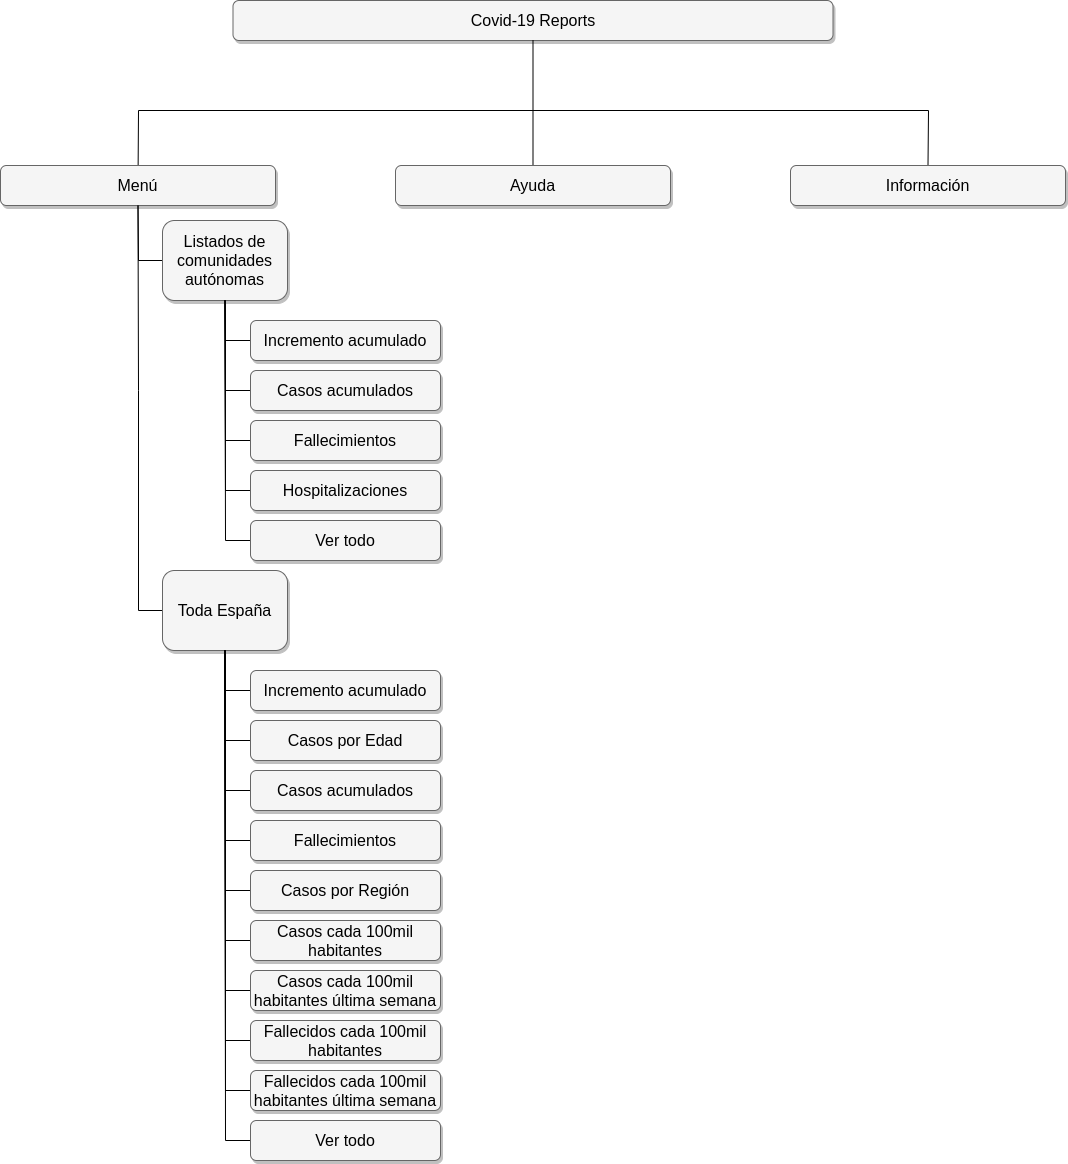
\includegraphics[width=0.9\textwidth]{img/sitemap}
	\caption{Sitemap del Bot.}
	\label{fig:sitemap}
\end{figure}

\subsection{Diseño del wireframe}

El \textbf{wireframe} es un boceto donde se representan visualmente de manera sencilla y estemática la estructura de una web. En este caso . Las Figuras \ref{fig:boceto1} a \ref{fig:boceto12} representan la estructura de \textbf{Covid-19 Reports}.

\begin{figure}[H]
	\centering
	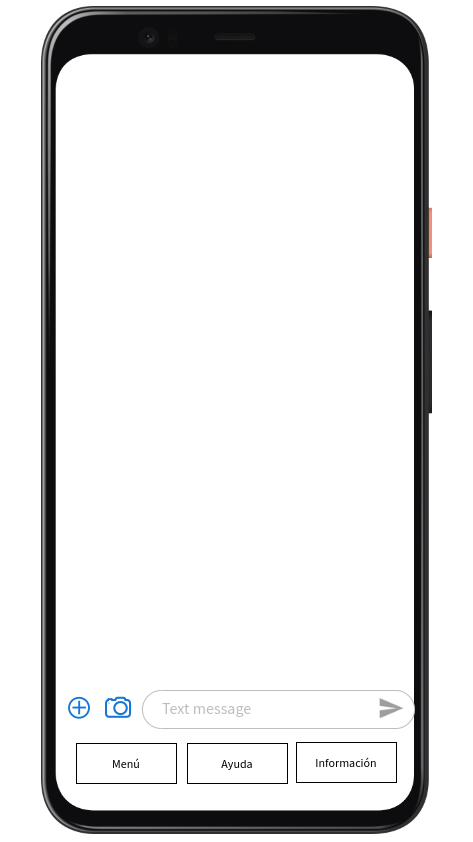
\includegraphics[width=0.75\textwidth]{img/boceto-inicio}
	\caption{Boceto de la pantalla principal.}
	\label{fig:boceto1}
\end{figure}

\begin{figure}[p]
	\centering
	\includegraphics[width=0.75\textwidth]{img/boceto-menú}
	\caption{Boceto Menú principal de selección.}
	\label{fig:boceto2}
\end{figure}

\begin{figure}[p]
	\centering
	\includegraphics[width=0.75\textwidth]{img/boceto-menú-comunidad}
	\caption{Boceto Menú Comunidad Autónoma.}
	\label{fig:boceto3}
\end{figure}

\begin{figure}[p]
	\centering
	\includegraphics[width=1.1\textwidth]{img/boceto-menú-incremento-acumulados}
	\caption{Boceto Menús Incremento y Casos acumulados.}
	\label{fig:boceto4}
\end{figure}

\begin{figure}[p]
	\centering
	\includegraphics[width=1.1\textwidth]{img/boceto-menú-fallecidos-hospitalizados}
	\caption{Boceto Menús Fallecidos y Hospitalizaciones.}
	\label{fig:boceto5}
\end{figure}

\begin{figure}[p]
	\centering
	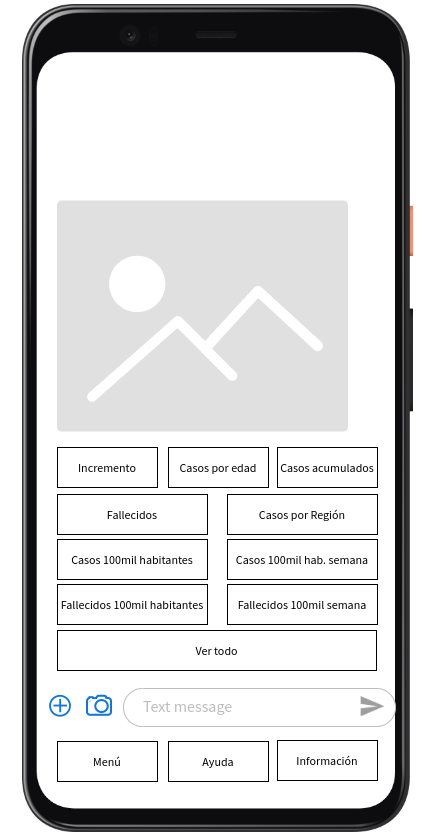
\includegraphics[width=1.1\textwidth]{img/boceto-menú-españa}
	\caption{Boceto Menú España.}
	\label{fig:boceto6}
\end{figure}

\begin{figure}[p]
	\centering
	\includegraphics[width=1.1\textwidth]{img/boceto-menú-es-incremento-edad}
	\caption{Boceto Menús Incremento y Casos por edad en España.}
	\label{fig:boceto7}
\end{figure}

\begin{figure}[p]
	\centering
	\includegraphics[width=1.1\textwidth]{img/boceto-menú-es-acumulados-fallecidos}
	\caption{Boceto Menús Casos acumulados y Fallecidos en España.}
	\label{fig:boceto8}
\end{figure}

\begin{figure}[p]
	\centering
	\includegraphics[width=1.1\textwidth]{img/boceto-menú-es-region-c100}
	\caption{Boceto Menús Casos por Región y Casos cada 100mil habitantes en España.}
	\label{fig:boceto9}
\end{figure}

\begin{figure}[p]
	\centering
	\includegraphics[width=1.1\textwidth]{img/boceto-menú-es-c100s-f100}
	\caption{Boceto Menús Casos cada 100mil hab. semana y Fallecidos cada 100mil habitantes en España.}
	\label{fig:boceto10}
\end{figure}

\begin{figure}[p]
	\centering
	\includegraphics[width=1.1\textwidth]{img/boceto-menú-es-f100s}
	\caption{Boceto Menú Fallecidos cada 100mil hab. semana en España.}
	\label{fig:boceto11}
\end{figure}

\begin{figure}[p]
	\centering
	\includegraphics[width=1.1\textwidth]{img/boceto-menú-ayuda-info}
	\caption{Boceto Menús Ayuda e Información.}
	\label{fig:boceto12}
\end{figure}

Como hemos visto, a lo largo de este capítulo se han mostrados los diferentes puntos del análisis del proyecto, los cuales nos serán útiles a la hora de llevar a cabo del mismo. En el próximo capítulo se muestra como se ha llevado a cabo la implementación del proyecto siguiendo las bases que se han desarrollado.